\section{Modelling of the Traction of the Metallic Strip}
As presented in the introduction, we know from a physical intuition that the traction in the metallic strip depends mainly on the difference of speed between the rolls, rather than on each of the speeds individually. For this reason, we only have to determine $Trac(s)$ as described in figure \ref{fig:tractionInput}, where $\omega_i$ is the speed of a motor, and $f$ is the traction of the metallic strip\footnote{Since we do not control the middle pair of rolls, we are not able to control the left and right traction separately. For this reason, in the following, we only care about controlling the right traction, which is denoted $f$ but sometimes $f_R$ in the matlab figures. With this setup, the left traction has roughly the same evolution as the right traction, multiplied by a coefficient slightly lower than $1$.}.
\begin{figure}[htbp]
\centering
\begin{tikzpicture}[auto, node distance=2cm,>=latex']
    % We start by placing the blocks
    \node [sum] (sum) {};
    \node [input, left of = sum, yshift = 1cm] (vr) {};
    \node [input, left of = sum, yshift = -1cm](vl) {};
    \node [sum, right of = sum, xshift = 1cm](addspeedsetpoint){};
    \node [input, below of = addspeedsetpoint](speed0){};
    \node [block, right of = addspeedsetpoint, xshift = 1cm](strip){$Trac(s)?$};
    \node [sum, right of = strip, xshift = 2cm](addtracsetpoint){};
    \node [input, below of = addtracsetpoint](tracsetpoint){};
    \node [output, right of = addtracsetpoint](trac){};

    % Once the nodes are placed, connecting them is easy.
    \draw [draw,->] (vr) node [yshift = 3mm]{$\omega_R$} -| node [pos = 0.9]{$+$} (sum);
    \draw [draw,->] (vl) node [yshift = 3mm]{$\omega_L$} -| node [pos = 0.9]{$-$} (sum);
    \draw [draw,->] (sum) -- node {$\Delta_\omega$} node[pos = 0.9]{$+$}  (addspeedsetpoint);
    \draw [draw,->] (speed0) -- node{${\Delta_\omega}_0$} node [pos = 0.9, right]{$-$} (addspeedsetpoint);
    \draw [draw,->]  (addspeedsetpoint) -- node{${\tilde{\Delta_\omega}}$} (strip);
    \draw [draw,->] (strip) -- node {$\tilde{f}$} node[pos = 0.9]{$+$} (addtracsetpoint);
    \draw [draw,->] (tracsetpoint) -- node {$f_0$} node[pos = 0.9, right]{$+$} (addtracsetpoint);
    \draw [draw,->] (addtracsetpoint) -- node {$f$} (trac);

\end{tikzpicture}
\caption{\label{fig:tractionInput}Simple gray-box model of the traction of the metallic strip}
\end{figure}

Furthermore, we also know that $Trac(s)$ should contain a close-to-perfect integrator. Indeed, if we increase $\Delta_\omega$ slightly from the setpoint ${\Delta_\omega}_0$, we expect the tension in the metallic strip to rise indefinitely until breakage. This is also confirmed by the experience: we observe that the system's response to a real world pulse is really close to a step, as showed in figure \ref{fig:tracImpulseResponse}.
\begin{figure}[htbp]
\centering
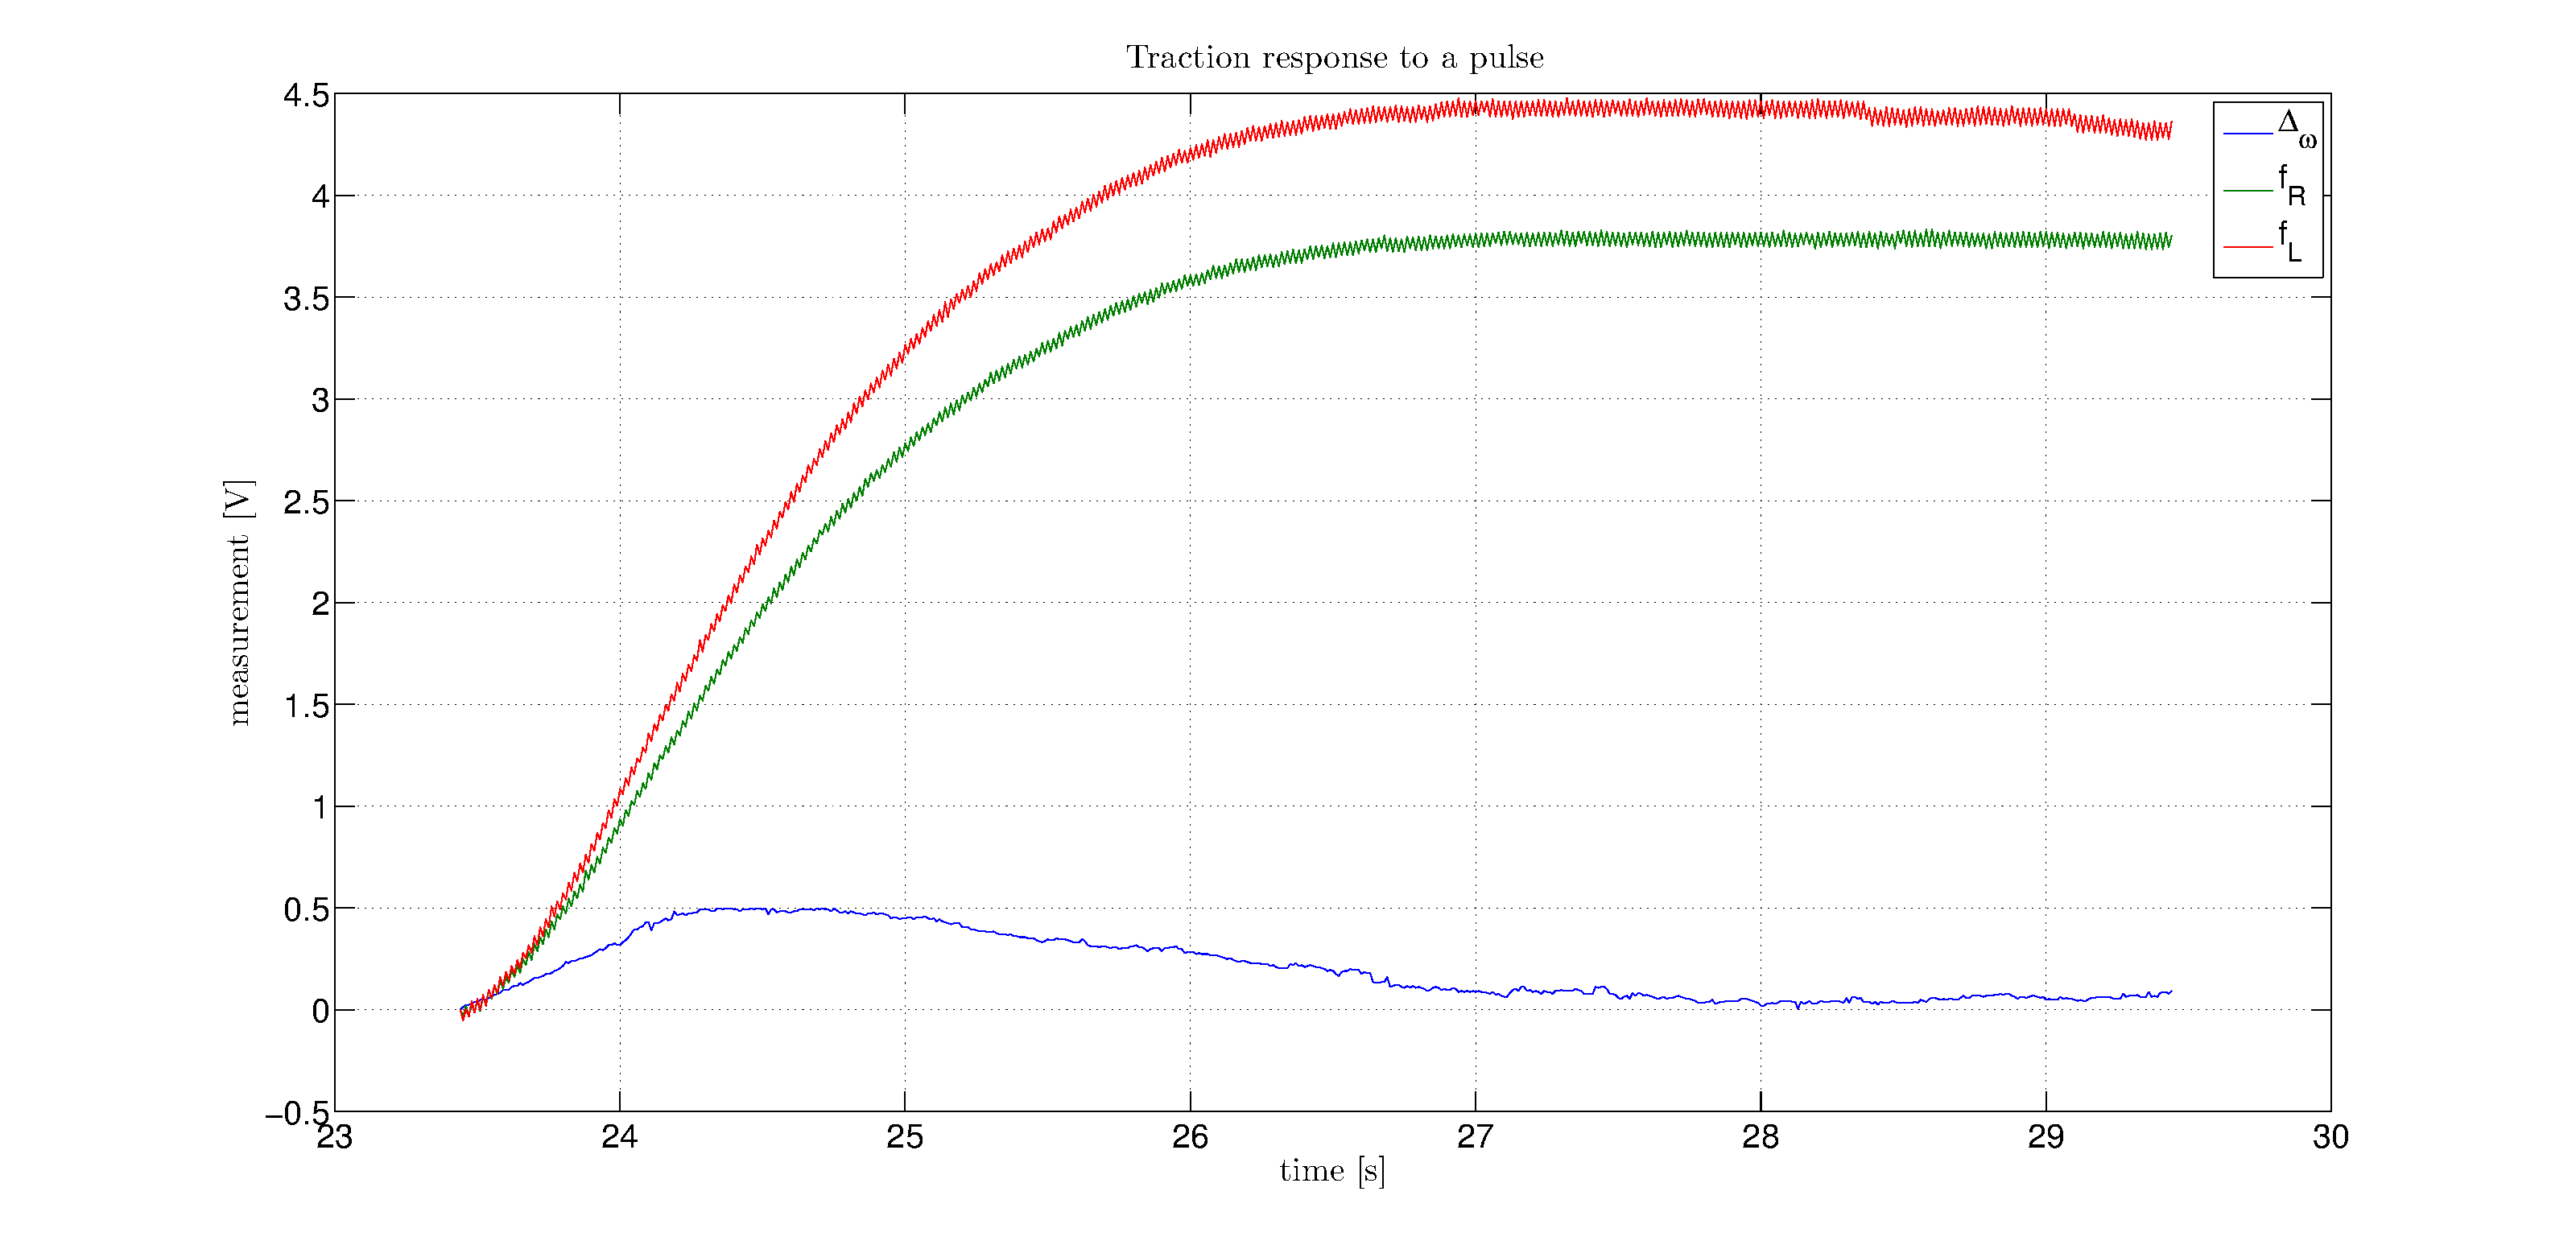
\includegraphics[width = \textwidth]{tractionPulse.pdf}
\caption{Traction response to a real world pulse\label{fig:tracImpulseResponse}}
\end{figure}
Finally, this is supported by a second order numerical approximation of the dynamics, which always yields a pole that is very close to zero.

However, this leads the rest of the optimisation problem to be badly conditioned. This means that the second pole is not reliably placed, and that the final result does not fit the real response accurately. Moreover, the obtained transfer function, with a very large $K$ and $p_2$, takes a long time to simulate with simulink.

To solve this, we refine our gray-box approximation by artificially introducing an integrator in the system we want to identify. We then compute its response to $\tilde{\Delta_\omega}(t)$ and try to determine the rest of the dynamics based on this new input and the observed response, as shown in figure \ref{fig:tractionGrayBox}, where $\frac{1}{s}\cdot H(s) = Trac(s)$. In the figure, we also use the fact that only $\omega_L$ is supposed to contribute to $\tilde{\Delta_\omega}$, since the master velocity is chosen steady. $\tilde{\omega_R}$ is thus considered as a disturbance.
\begin{figure}[htbp]
\centering
\begin{tikzpicture}[auto, node distance=2cm,>=latex']
    % We start by placing the blocks
    \node [input](input){};
    \node [sum, right of = input, xshift = 0.5cm](add){};
    \node [input, above of = add, yshift = -0.8cm](disturb){};
    \node [square, right of = add, xshift = 0cm](integrator){$\frac{1}{s}$};
    \node [block, right of = integrator, xshift = 2.5cm](strip){$H(s)?$};
    \node [output, right of = strip](trac){};

    % Once the nodes are placed, connecting them is easy.
    \draw [draw,->]  (input) -- node{${\tilde{\omega_L}}$} node[pos = 0.9, below]{$-$} (add);
    \draw [draw,->]  (disturb) -- node[pos = 0.2]{$d$} node[pos = 0.9]{$+$} (add);
    \draw [draw,->]  (add) -- (integrator);
    \draw [draw,->]  (integrator) -- node{${\int^t_0\tilde{\omega_L}}dt$} (strip);
    \draw [draw,->] (strip) -- node {$\tilde{f}$} (trac);
\end{tikzpicture}
\caption{Gray-box model of the traction of the metallic strip\label{fig:tractionGrayBox}}
\end{figure}

Fitting a simple first order transfer function to $H(s)$ is not easy because the dynamics between $\int_0^t\tilde{\omega_L}(t)$ and $f(t)$ is very fast, as shown in figure \ref{fig:tractionPulseStep}. This leads to very large poles which are not well approximated and difficult to simulate, as experienced previously.
\begin{figure}[htbp]
\centering
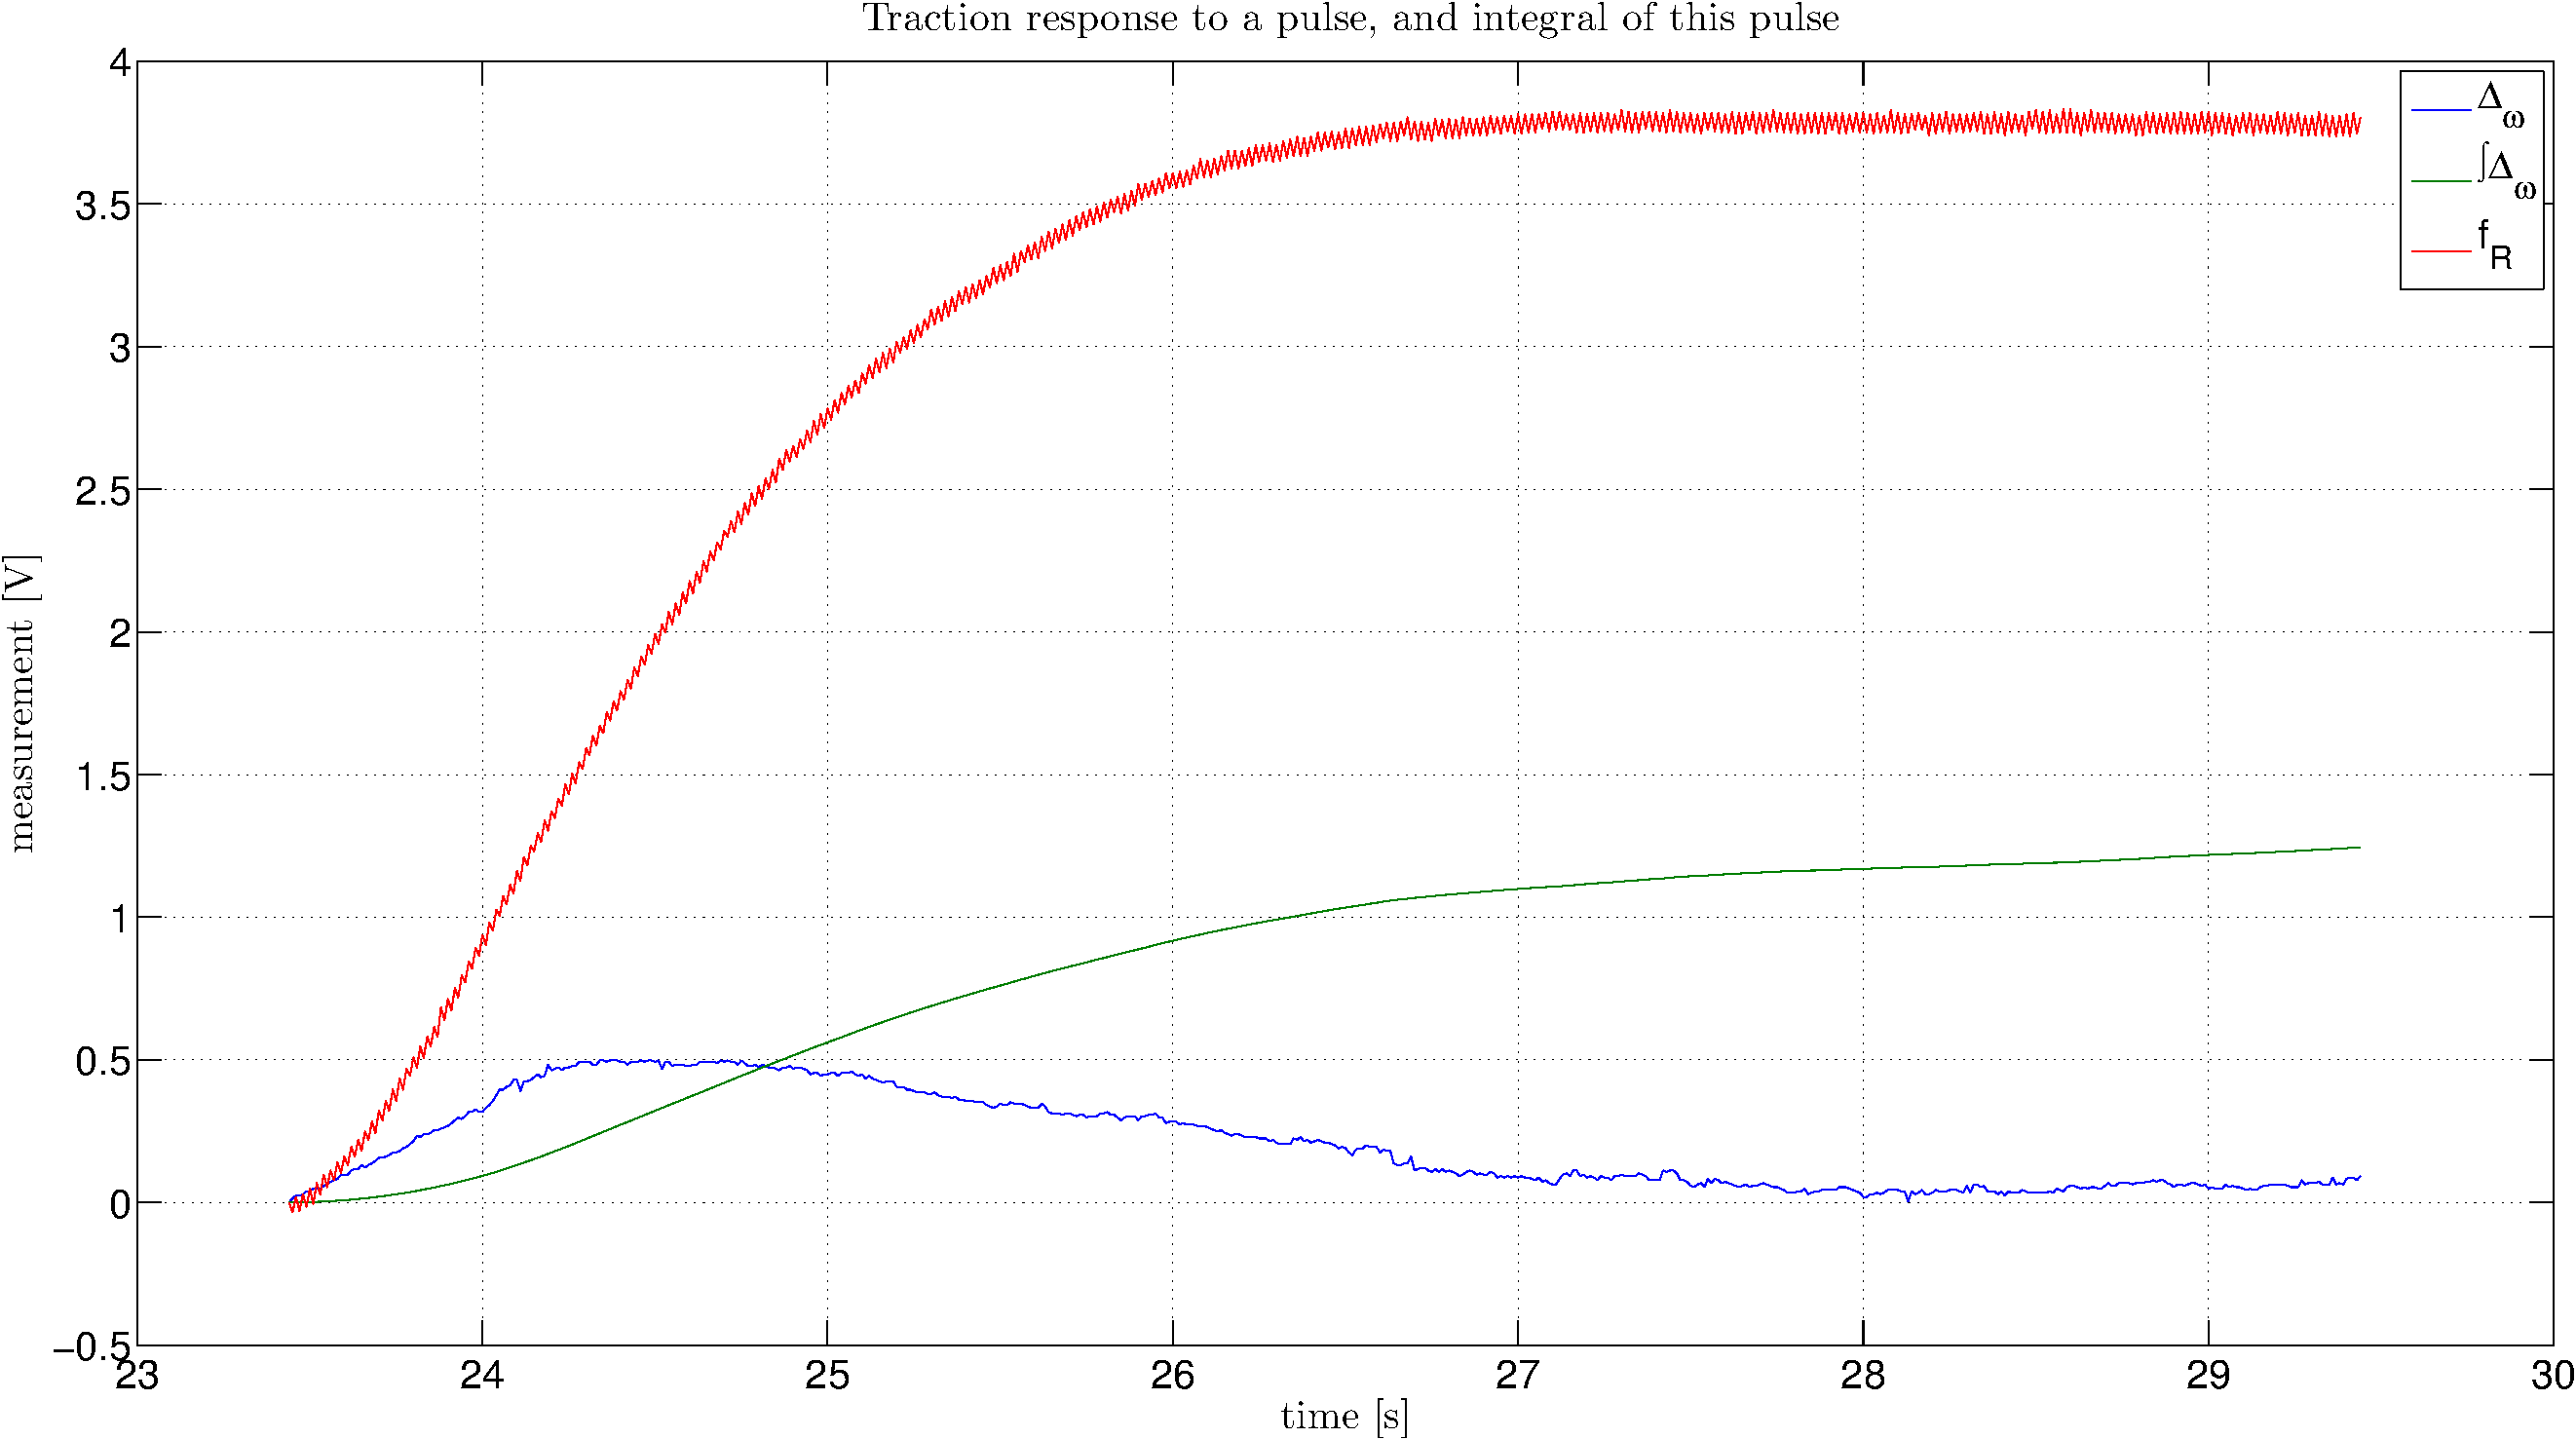
\includegraphics[width = \textwidth]{tractionPulseStep.pdf}
\caption{Right traction response to a pulse and output of the intermediate integrator\label{fig:tractionPulseStep}}
\end{figure}

To solve this, we try to fit $H(s)$ with a transfer function of the form $K\frac{s-z_1}{s-p_2}$, because the introduction of a zero speeds up a step response, which would bring $p_2$ reasonably closer to the origin. The result is shown in figure \ref{fig:tracFit}, where we see that $Trac(s)$ as given in equation \ref{eqn:tracS} seems to fit the experience very well.
\begin{align*}
  H(s) &= 13.096\cdot\frac{s+0.9221}{s+4.063}\\
  Trac(s) &= 13.096\cdot\frac{s+0.9221}{s(s+4.063)}\numberthis\label{eqn:tracS}
\end{align*}
\begin{figure}[htbp]
\centering
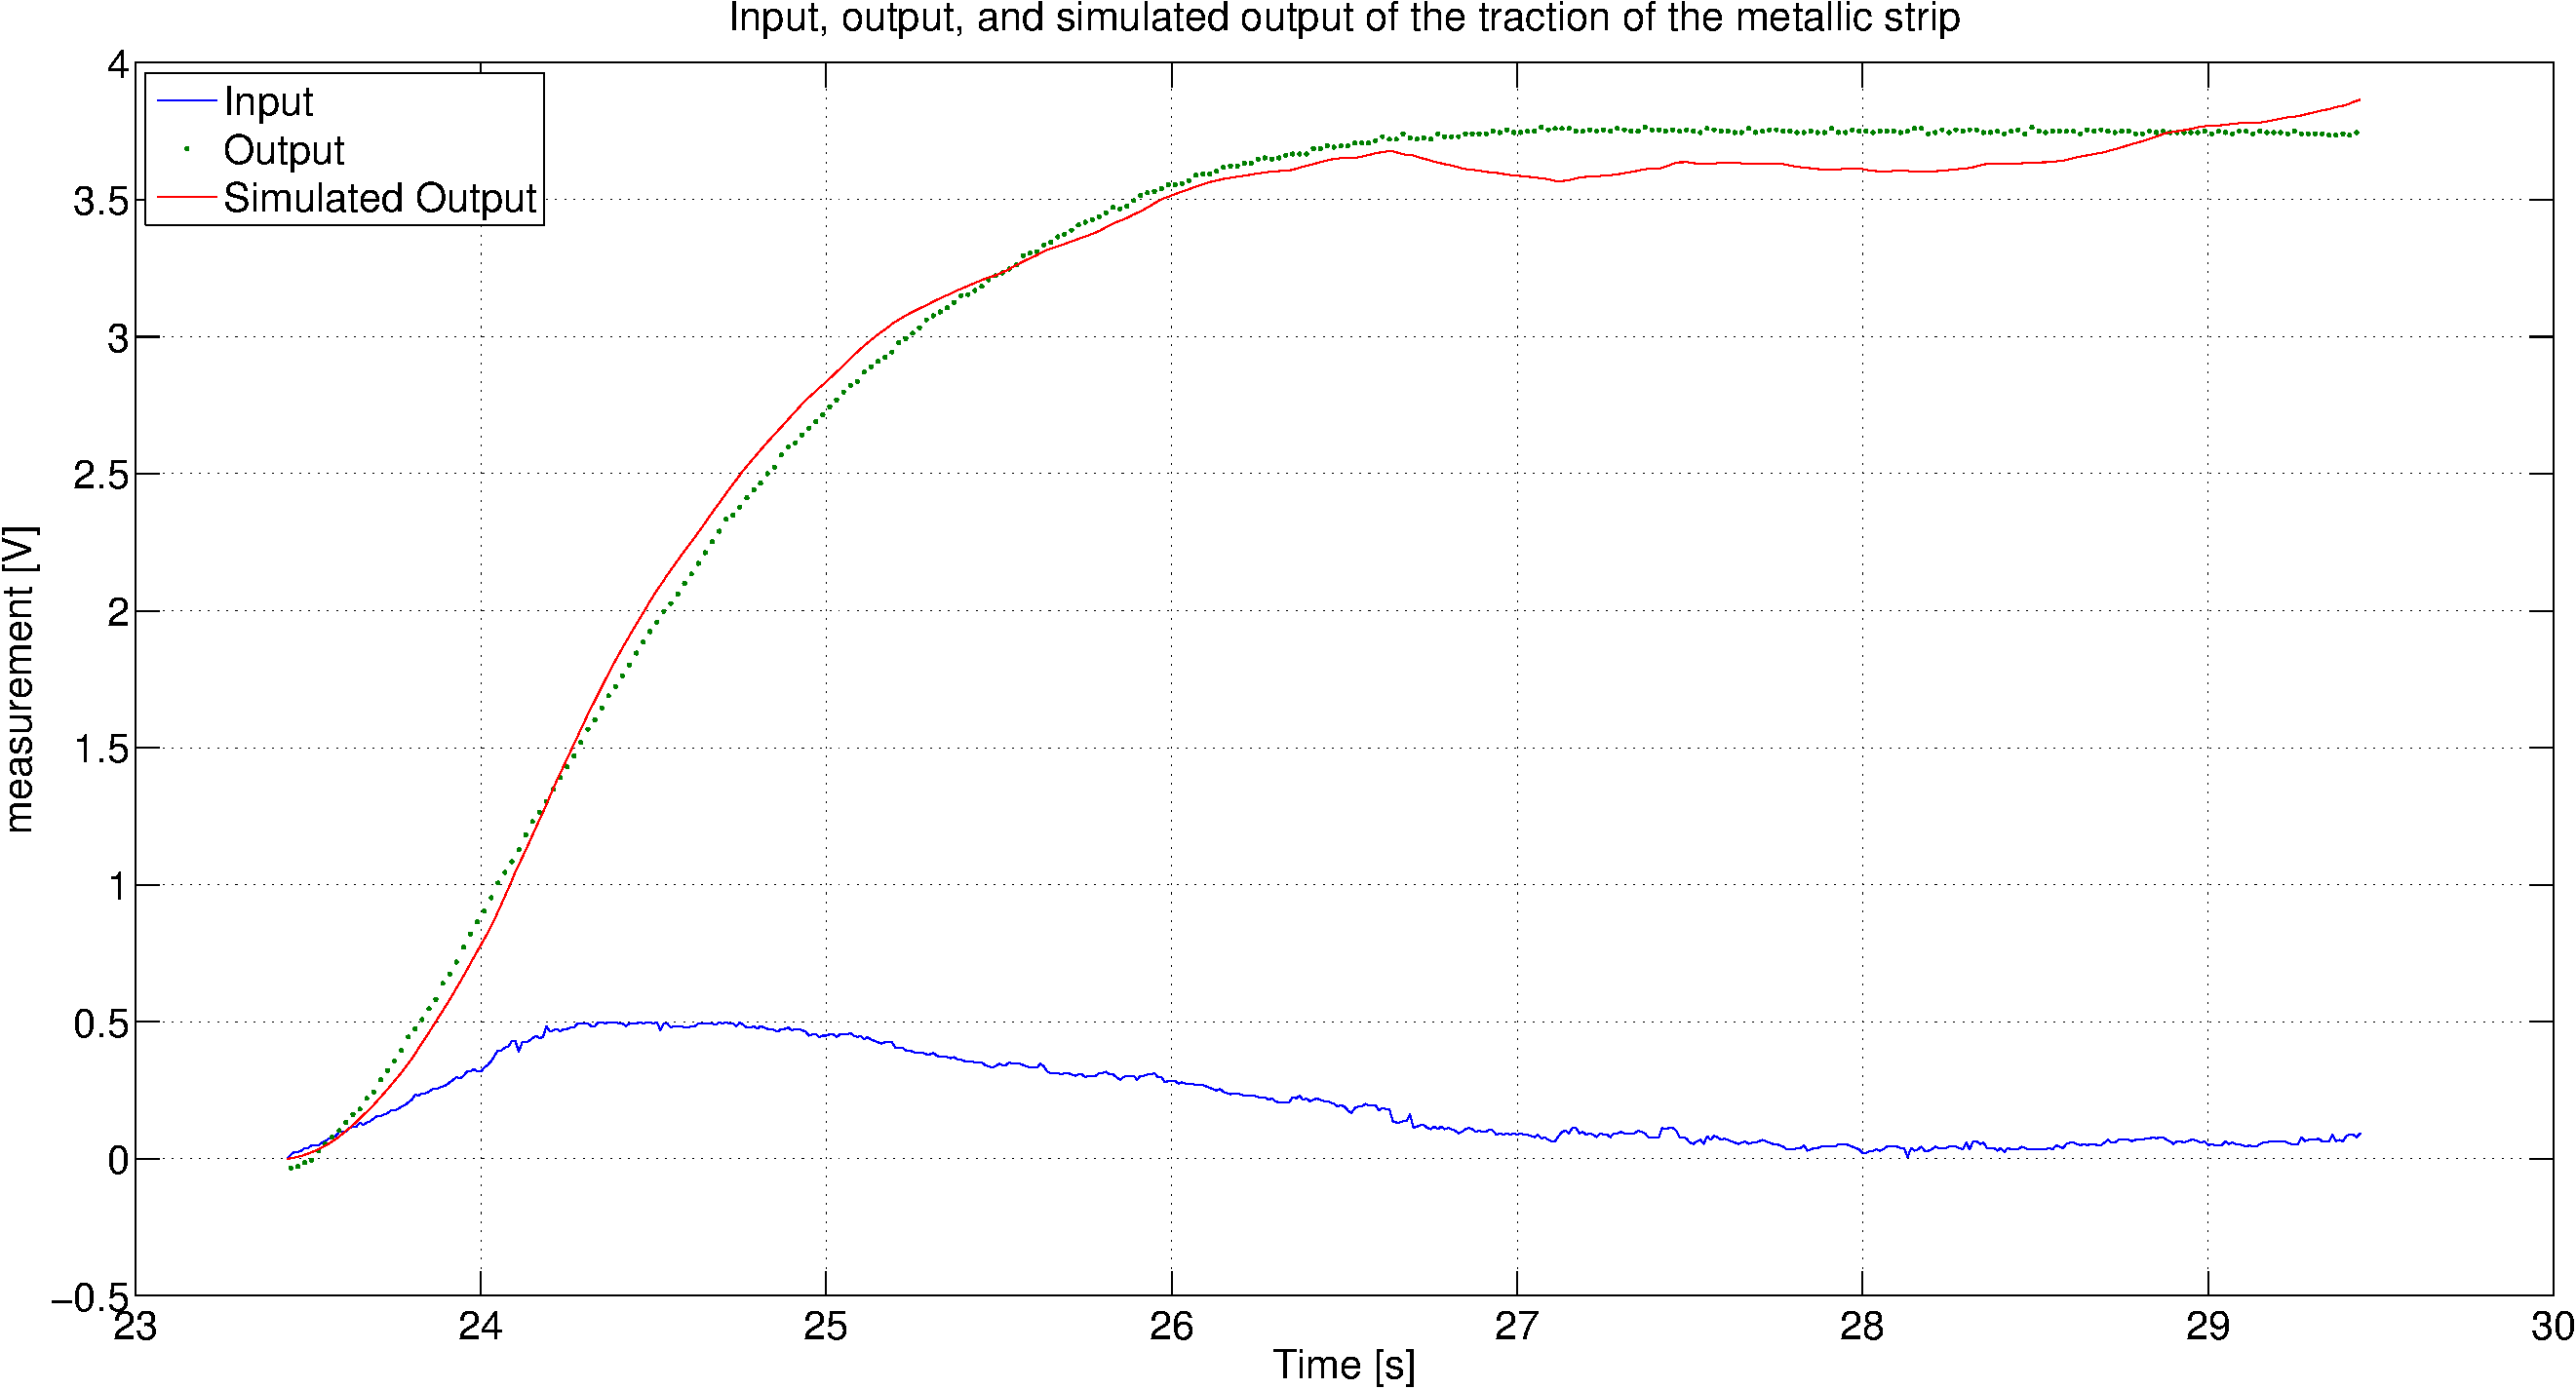
\includegraphics[width = \textwidth]{tracFit.pdf}
\caption{Input, output, and simulated output of the traction of the metallic strip\label{fig:tracFit}}
\end{figure}

\section{Control of the Traction}
\subsection{Simple P Controller}
Since there already is an integrator in the system, and since we do not have specifications on the transient response, we first try to control the traction with a simple P~controller, which should provide asymptotic stability and zero steady-state error. Figure \ref{fig:tracRLocus}
\begin{figure}[htbp]
  \centering
  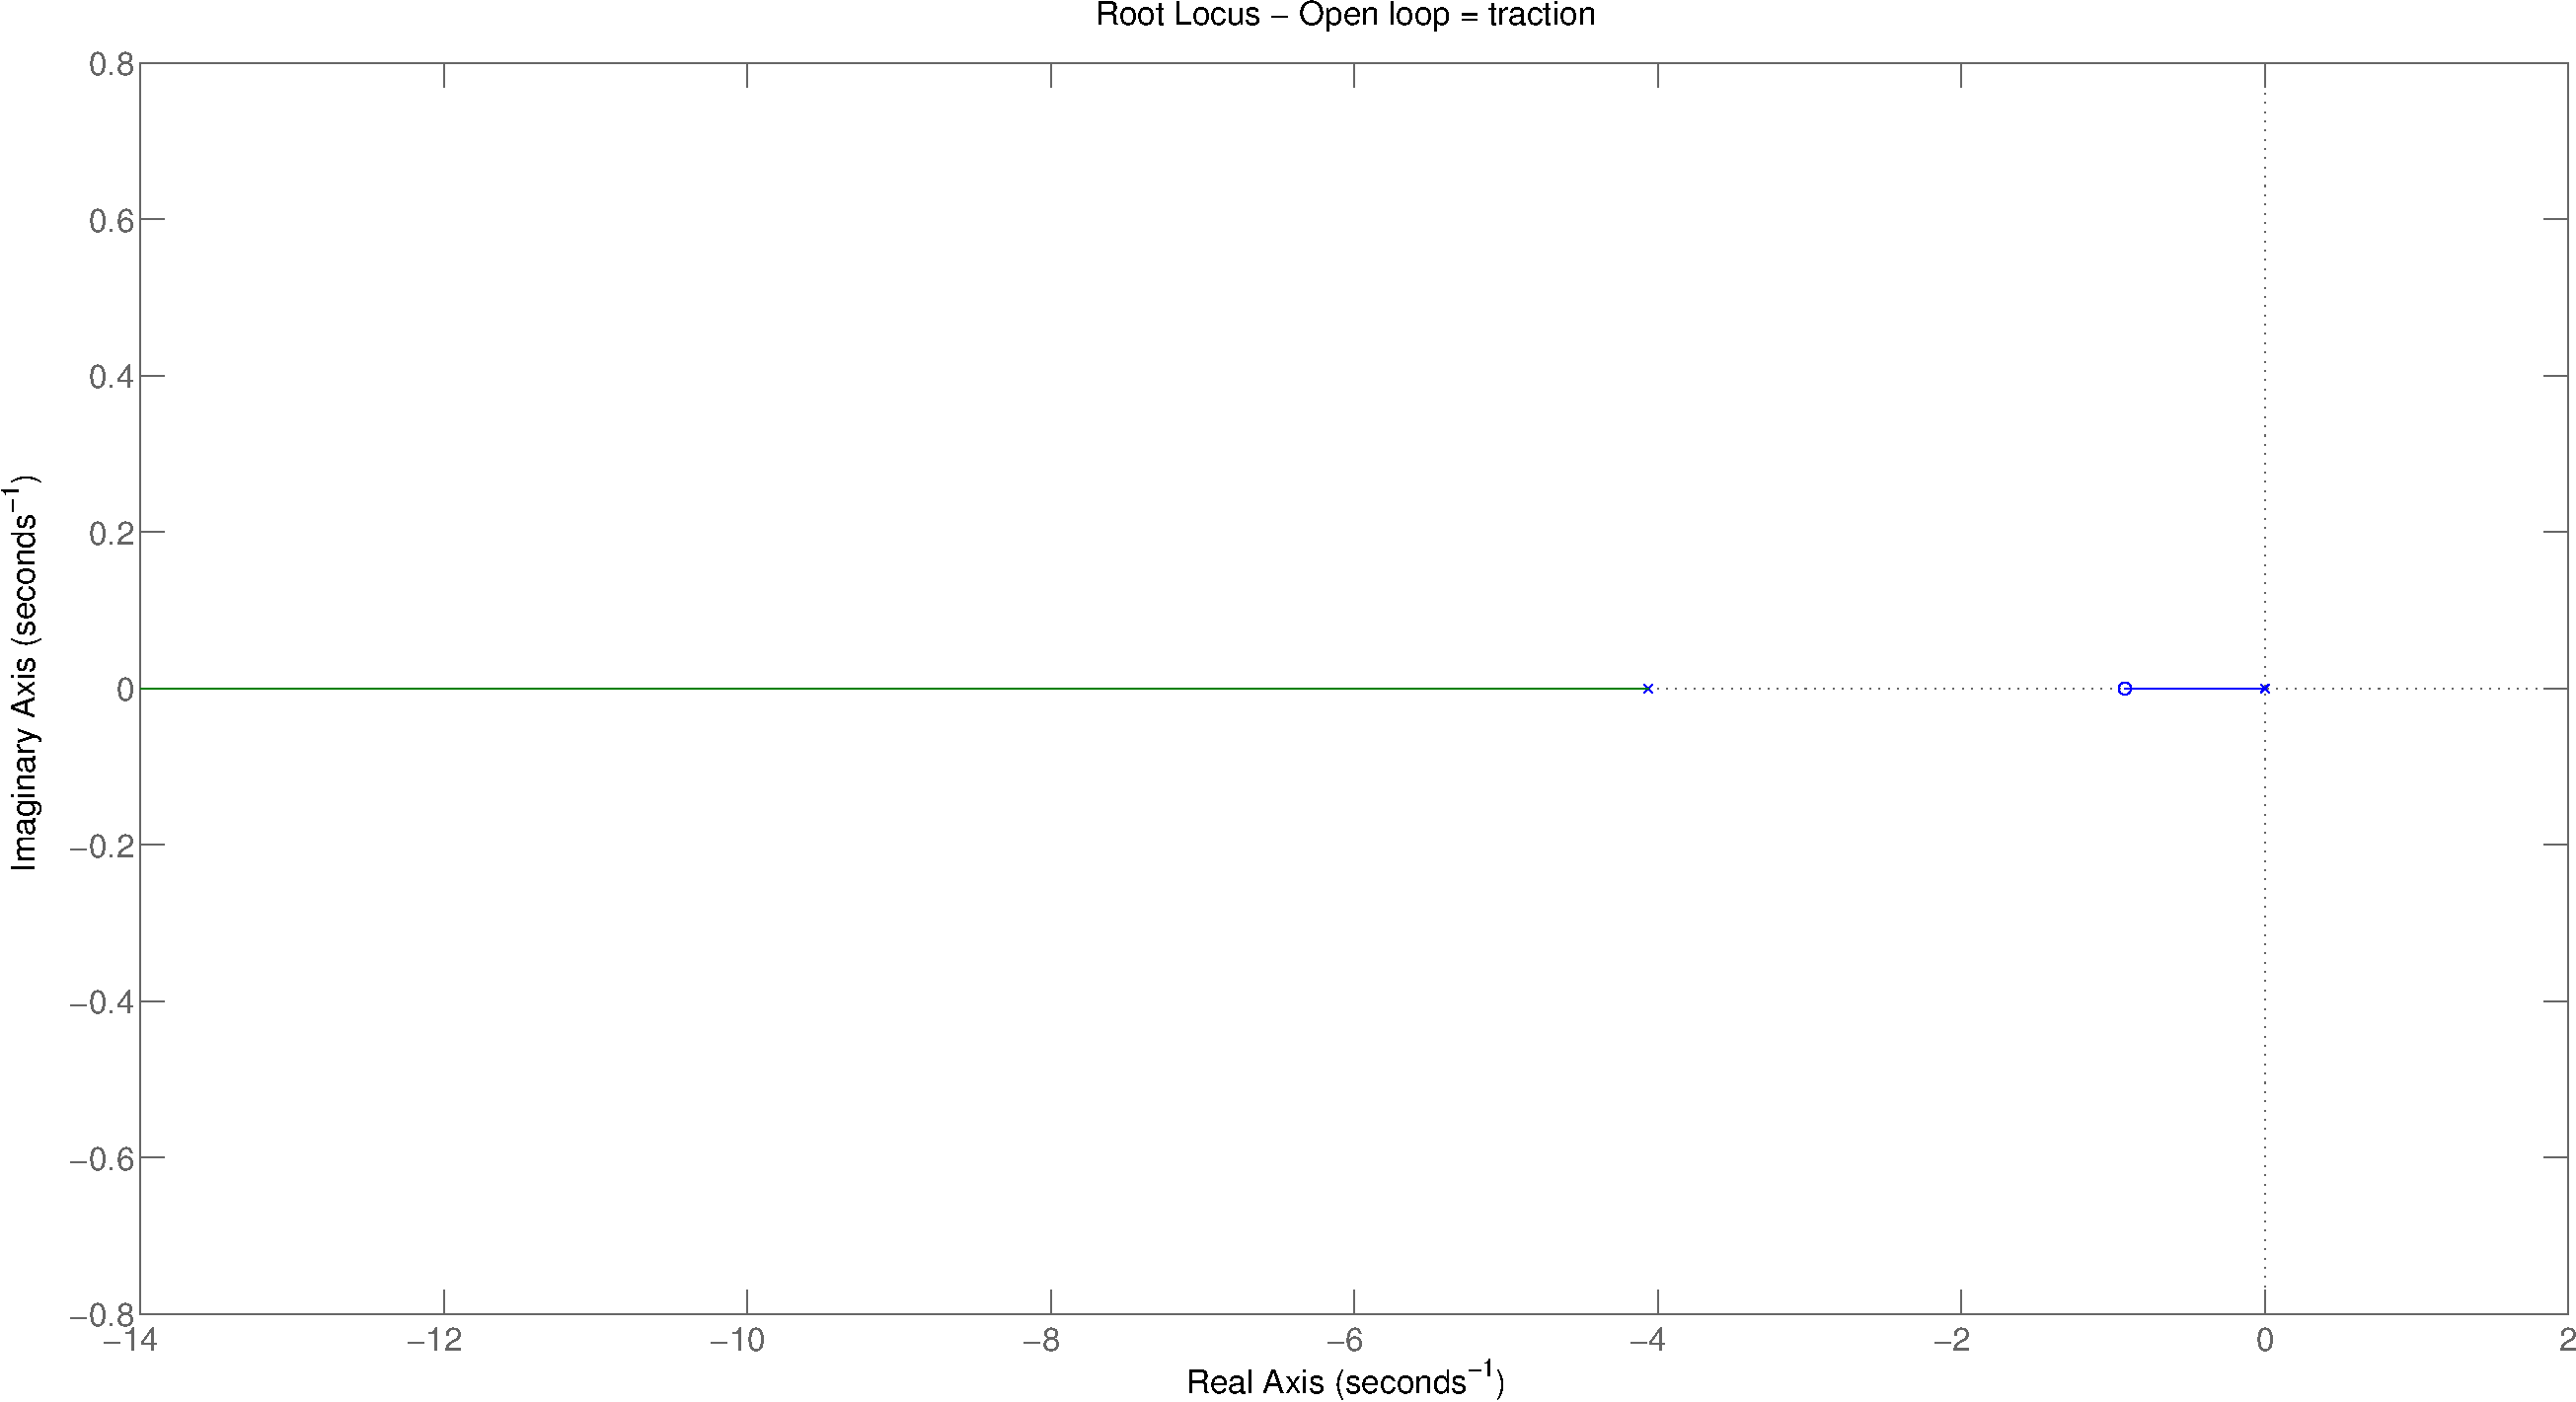
\includegraphics[width = \textwidth]{rlocus_trac.pdf}
  \caption{Root locus of the traction\label{fig:tracRLocus}}
\end{figure}
shows the root locus of the traction for this controller, with the approximation that the inner slave speed loop is fast enough to be considered perfectly transparent. The root locus shows that $k_P < 0$\footnote{The $\tilde{\omega_L}$ input is inverting, as shown in figure \ref{fig:tractionGrayBox}} can be theoretically chosen as high as desired while keeping the closed-loop poles on the real axis.

Figure \ref{fig:simuPTot}
\begin{figure}[htbp]
  \centering
  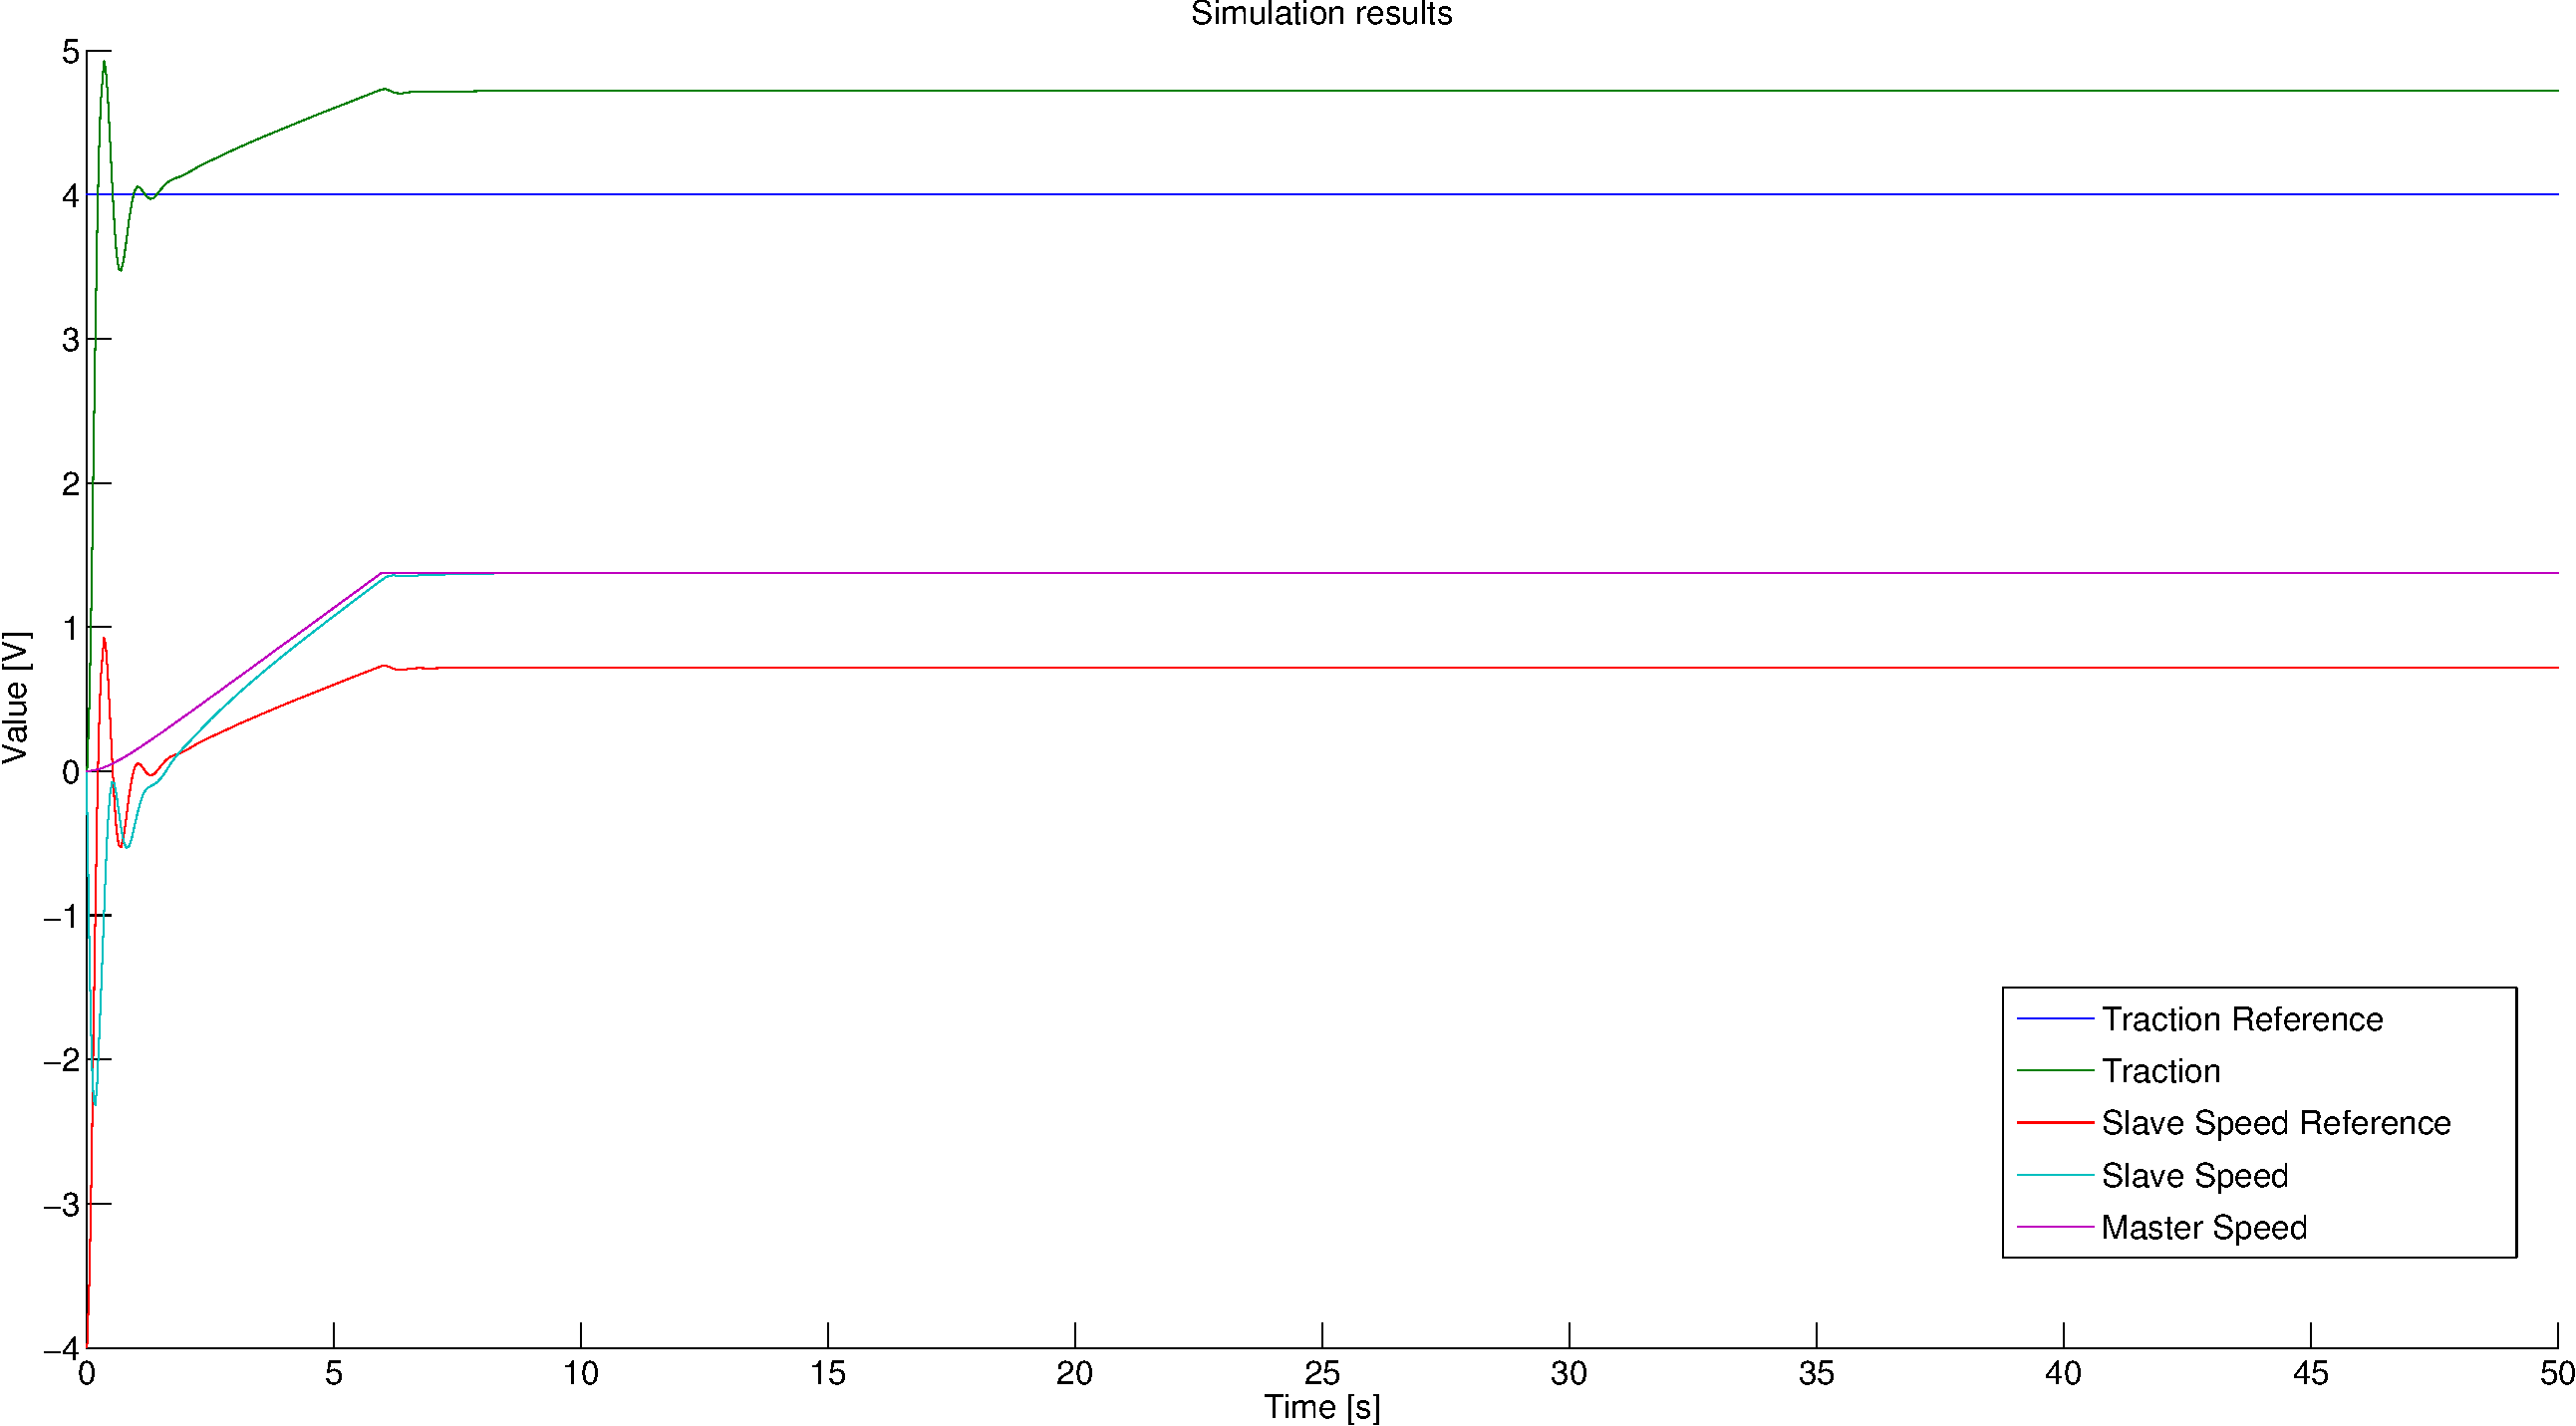
\includegraphics[width = \textwidth]{simu_P_tot.pdf}
  \caption{Simulation of the rolling mill operation with a P controller on the traction\label{fig:simuPTot}}
\end{figure}
shows the closed-loop traction response to a constant reference, with an arbitrary gain of $-1$, as simulated by simulink. First, we observe that the closed-loop poles are not real, which is due to non linearities and higher order effects. More importantly, we see that the steady-state error is not cancelled.

Comparing the measured traction and the master speed, we observe that the initial ramp on the master motor is not compensated. In steady state, the master speed also creates an offset on the traction. This is because the right velocity is actually a disturbance, as was shown in figure \ref{fig:tractionGrayBox}. This disturbance is not rejected because the integrator is in the plant, and not in the controller.

To achieve perturbation rejection, an integrator should be added to the controller. However, this is not a good solution as is, because the open loop would then contain two integrators. This would greatly reduce the phase margin and thus make the closed loop system nearly unstable and slow its response down.

\subsection{Second Loop: PI Controller}
Rather then adding an integrator to the existing controller, we can add a second external loop with a PI, as shown in figure \ref{fig:simulinkTot}
\begin{figure}[htbp]
  \centering
  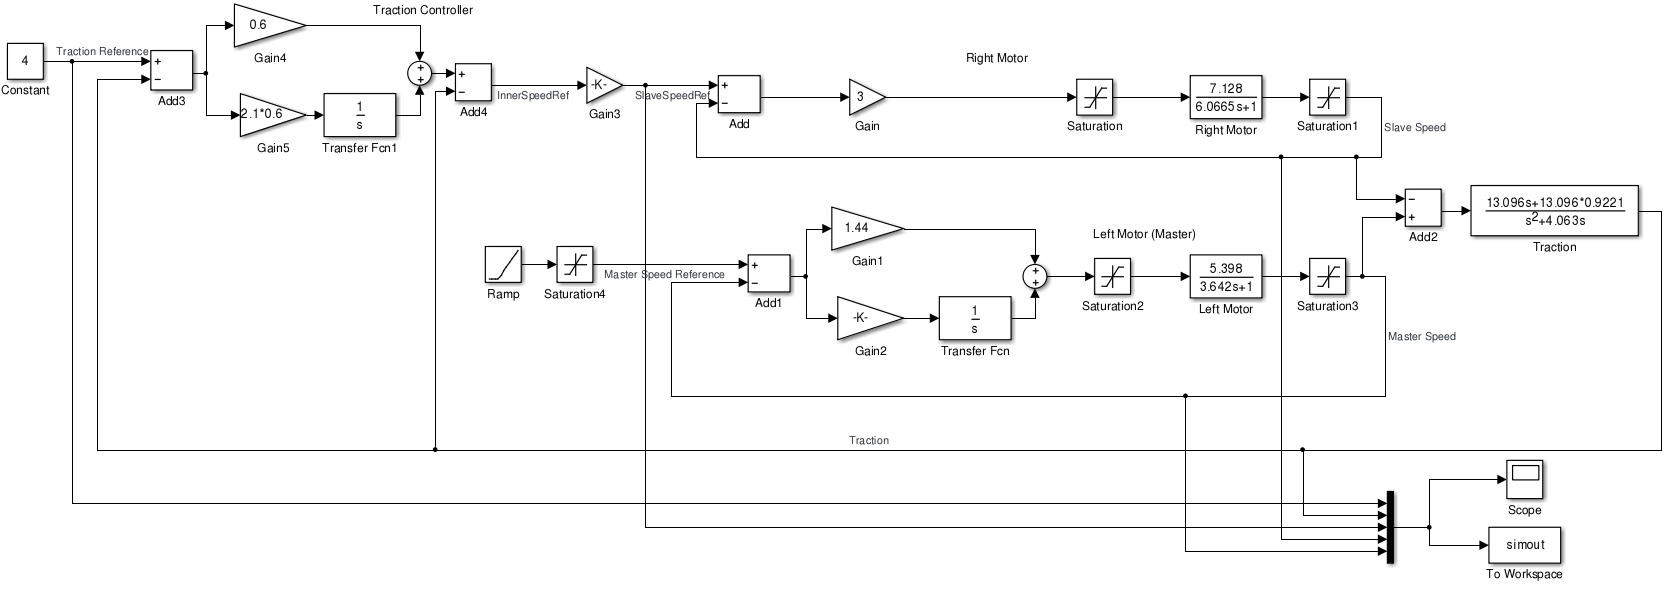
\includegraphics[width = \textwidth]{simulink.png}
  \caption{Final controller architecture\label{fig:simulinkTot}}
\end{figure}
,to achieve perturbation rejection while preserving the phase margin. In this section, the reasoning behind this second loop will be explained. In the following
